\documentclass[../DS10.tex]{subfiles}%
\graphicspath{{./figures/}}%

% \subimport{/home/nora/Documents/Enseignement/Prepa/bpep/exercices/DS/titrage_CO2/}{sujet.tex}%

\begin{document}%
\section[32]"E"{Étude cristallographique de la chromite\ifcorrige{~\small\textit{(D'après Banque PT 2023)}}}

\enonce{%
	Le trioxyde de chrome est un oxydant fort, très utilisé au laboratoire. Il est
	obtenu industriellement à partir de la chromite de formule $\ce{Fe_xCr_yO_z}$
	qui est le principal minerai du chrome. Nous nous intéressons à la structure
	de la chromite pour déterminer $x$, $y$ et $z$ ainsi que le degré d’oxydation
	(t) du chrome dans le minerai.
	\bigbreak
	La chromite $\ce{Fe_xCr_yO_z}$ cristallise dans une structure que l’on peut
	décrire de la façon suivante : les ions $\ce{O^{2-}}$ forment un réseau cubique
	à faces centrées (cfc), les ions $\ce{Fe^{2+}}$ occupent certains sites
	tétraédriques et les ions $\ce{Cr^{t+}}$ occupent certains sites octaédriques.
}%

\QR[5]{%
	Représenter la maille conventionnelle du réseau cubique à faces centrées formé
	par les anions $\ce{O^{2-}}$. Indiquer la position des sites tétraédriques et
	des sites octaédriques dans un réseau cubique à faces centrées. Préciser sur
	le schéma la position d’un site tétraédrique et d’un site octaédrique.
}{%
	~
	\smallbreak
	\vspace{-15pt}
	\begin{isd}[righthand ratio=.4, interior hidden]
		\begin{itemize}
			\item[bl](\pt{1}){Site T}: On trouve les sites tétraédriques aux centres
			les petits cubes d'arêtes $a/2$~;
			\item[bl](\pt{1}){Site O}: On trouve les sites octaédriques au milieu des arêtes,
			ainsi qu'un au centre du cube.
		\end{itemize}
		\tcblower
		\begin{center}
			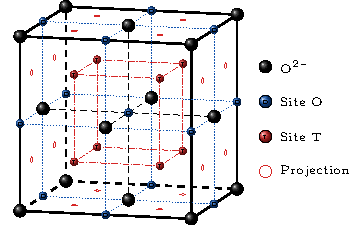
\includegraphics[width=\linewidth]{maille}
			\captionsetup{justification=centering}
			\captionof{figure}{\\Schéma. \protect\pt{1}+\protect\pt{1}+\protect\pt{1}}
		\end{center}
		\vspace{-30pt}
	\end{isd}
}%

\QR[2]{%
	Déterminer le nombre d'ions $\ce{O^{2-}}$ par maille.
}{%
	Il y a 8 ions oxyde aux sommets, qui comptent pour 1/8, et 6 aux centres des
	faces, qui comptent pour 1/2, soit
	\[
		\boxed{
			N_{\ce{O^{2-}}} \stm{=}
			8 \times \frac{1}{8} + 6 \times \frac{1}{2} \stm{=} 4
		}
	\]
}%

\QR[4]{%
	Déterminer le nombre de sites tétraédriques et le nombre de sites octaédriques
	par maille. Sachant que les ions $\ce{Fe^{2+}}$ occupent 1/8 des sites
	tétraédriques et les ions $\ce{Cr^{t+}}$ occupent la moitié des sites
	octaédriques, déterminer le nombre d'ions $\ce{Fe^{2+}}$ et $\ce{Cr^{t+}}$ par
	maille.
}{%
	\begin{itemize}
		\item[bl](\pt{1}){Site T}: Il y a 8 petits cubes d'arête $a/2$, et les
		sites T appartiennent en propre à la maille~: $N_T = 8$~;

		\item[bl](\pt{1}){Site O}: Les arêtes comptent pour 1/4 et le centre pour
		1~: $N_O = 12 \times 1/4 + 1 = 4$
	\end{itemize}
	Ainsi,
	\[
		N_{\ce{Fe^{2+}}} = \frac{1}{8} \times N_T
		\Lra
		\boxed{N_{\ce{Fe^{2+}}} \stm[-1]{=} 1}
		\qqet
		N_{\ce{Cr^{t+}}} = \frac{1}{2} \times N_O
		\Lra
		\boxed{N_{\ce{Cr^{t+}}} \stm[-1]{=} 2}
	\]
}%

\QR[3]{%
	En déduire la formule de la chromite $\ce{Fe_xCr_yO_z}$. Quelle est la formule
	de l'ion du chrome dans le cristal~?
}{%
	On en déduit la formule $\boxed{\ce{FeCr_2O_4}}$ \pt{1}. On trouve la charge
	du chrome par neutralité électrique~:
	\[
		N_{\ce{Fe^{2+}}} \times q_{\ce{Fe^{2+}}} +
		N_{\ce{Cr^{t+}}} \times q_{\ce{Cr^{t+}}} +
		N_{\ce{O^{2-}}} \times q_{\ce{O^{2-}}} \stm[-1]{=} 0
		\Lra
		1 \times 2 + 2 \times t + 4 \times (-2) = 0
		\Lra
		\boxed{t = 3}
		\Ra
		\boxed{\ce{Cr^{3+}}} \pt{1}
	\]
}%

\QR[8]{%
	Le paramètre de la maille vaut $a = \SI{420}{pm}$, le rayon ionique de l'ion
	$\ce{O^{2-}}$ vaut $r(\ce{O^{2-}}) = \SI{140}{pm}$. Rappeler les conditions de
	stabilité d'un crital ionique, puis calculer le rayon du plus gros cation que
	l'on puisse insérer dans un site octaédrique. Calculer de même le rayon du
	plus gros cation que l'on puisse insérer dans un site tétraédrique. On
	précise que dans la structure les ions $\ce{O^{2-}}$ ne sont pas tangents.
}{%
	Dans un cristal ionique, il y a tangence cation/anion \pt{1} et non-contact
	anion/anion \pt{1}.
	\smallbreak
	\begin{itemize}
		\item[b]{Site T}: Il y a tangence sur la \textbf{grande diagonale}
		\pt{1} des petits cubes, soit
		\begin{gather*}
			r_T + r_{\ce{O^{2-}}} = \frac{a \sqrt{3}}{4}
			\Lra
			\boxed{r_T \stm{=} \frac{a \sqrt{3}}{4} - r_{\ce{O^{2-}}}}
			\\\AN
			\xul{r_T \stm{\approx} \SI{38.5}{pm}}
		\end{gather*}
		\item[b]{Site O}: Il y a tangence sur la \textbf{une arête}
		\pt{1} du cube, soit
		\begin{gather*}
			r_O + r_{\ce{O^{2-}}} = \frac{a}{2}
			\Lra
			\boxed{r_O \stm{=} \frac{a}{2} - r_{\ce{O^{2-}}}}
			\\\AN
			\xul{r_O \stm{\approx} \SI{70}{pm}}
		\end{gather*}
	\end{itemize}
}%

\QR[5]{%
	En réalité, les rayons ioniques sont les suivants~: $r (\ce{Fe^{2+}}) =
		\SI{76}{pm}$ et $r (\ce{Cr^{t+}}) = \SI{61.5}{pm}$. Comparer ces valeurs aux
	valeurs calculées à la question précédente. Commenter.
}{%
	\begin{itemize}
		\item[b]{Site T}:
		$r_{\ce{Fe^{2+}}} \stm[-1]{>} r_{T,\mathrm{max}}$, ce qui est impossible~!
		Soit il y a \textbf{déformation} \pt{1} de la structure par les ions fer,
		soit le modèle des \textbf{sphères dures} \pt{1} est à remettre en cause.
		Les liaisons ne seraient pas entièrement ioniques, mais pourraient être en
		partie covalente.
		\item[b]{Site O}:
		$r_{\ce{Cr^{3+}}} \stm[-1]{<} r_{O,\mathrm{max}}$, donc il n'y a \textbf{pas
			de contact} $\ce{O^{2-}}-\ce{Cr^{3+}}$ \pt{1}
	\end{itemize}
}%

\QR[3]{%
	Rappeler la définition puis \textbf{établir} la formule de la masse volumique
	de la chromite en fonction, notamment, des masses molaires des éléments.
}{%
	On a, avec $m = M/\Nc_A$ \pt{1}
	\[
		\rho \stm{=} \frac{\text{masse des ions}}{\text{volume maille}}
		\Lra
		\rho \stm{=} \frac{\sum_i N_i m_i}{a^3}
		\Lra
		\boxed{\rho \stm{=} \frac{M_{\ce{Fe}} + 2 M_{\ce{Cr}} + 4 M_{\ce{O}}}{\Nc_A \times a^3}}
	\]
}%

\QR[2]{%
	Rappeler la définition puis établir l'expression de la compacité en fonction
	du rayon des ions et du paramètre de maille $a$.
}{%
	On a
	\[
		C \stm{=} \frac{\text{volume des ions}}{\text{volume maille}}
		\Lra
		\boxed{C \stm{=} \frac{4}{3}\pi \times \frac{r_{\ce{Fe^{2+}}}^3 + 2
				r_{\ce{Cr^{3+}}}^3 + 4 r_{\ce{O^{2-}}}^3}{a^3}}
	\]
}%

\end{document}%
